\chapter{Методика разработки и исследования динамики систем управления бортовыми оптико-электронными приборами с применением информационных технологий} \label{ch:ch2}

В настоящее время наиболее распространены в народном хозяйстве и военной технике комплексированные оптико - электронные системы (КОЭП) визуализации, включающие в себя каналы наблюдения и зондирования в широком спектре волн оптического диапазона \cite[]{Tarasov},\cite[]{Belyakov},\cite[]{Karpov},\cite[]{Torshina}. Появление на рынке матричных фотоприемников расширило возможности КОЭП и К(комплексов). Несмотря на интенсивное развитие   теории и методов расчета и совершенствование бортовых автоматических КОЭП и К  возникают ряд вопросов, влияющих на качество получаемой оптической информации, в частности – это вопросы динамики и качества управления и увязки их с оптическими характеристиками каналов визуализации \cite[]{Belyakov},\cite[]{Karpov}, \cite[]{Baloev16}, \cite[]{Karpov17}.

Рассматриваются алгоритмы методики разработки и исследования динамики систем виброзащиты и управления бортовыми оптико- электронными приборами в виде десяти последовательных интерактивных замкнутых процедур от анализа технического задания до испытаний на борту.

Оптико-электронные приборы (ОЭП) авиационного, морского, наземного и космического базирования нашли широкое применение при выполнении задач наблюдения и охраны, в том числе при решении народнохозяйственных задач и задач обороны и безопасности.

В настоящее время широко рекламируются комплексированные ОЭП визуализации, включающие в себя каналы наблюдения и зондирования в широком спектре волн оптического диапазона, для применения в народном хозяйстве и военной технике \cite[]{Tarasov},\cite[]{Belyakov}, \cite[]{Torshina}, \cite[]{Ivanov18}. Появление на рынке матричных фотоприемников расширило возможности ОЭП и комплексов. Несмотря на интенсивное развитие   теории и методов расчета и совершенствование бортовых автоматических ОЭП возникает ряд вопросов, влияющих на качество получаемой оптической информации, в частности – это вопросы динамики и качества управления и увязки их с характеристиками каналов визуализации \cite[]{Tarasov},\cite[]{Belyakov}, \cite[]{Baloev16}, \cite[]{Karpov17}, \cite[]{Gerasin19}. Ниже в развитие работы \cite[]{Tarasov} рассматривается методика разработки и исследования систем автоматического управления (САУ) и виброзащиты (СВ) ОЭП с использованием замкнутых процедур исследования от разработки математических моделей до испытаний на борту носителя.


\section{Методика разработки и исследования динамики} \label{sec:ch2/sec1-}


Разработка СВ и САУ ОЭП начинается с выбора приемлемого варианта. Для этого решается много критерийная задача оптимизации с учетом ряда противоречивых технико-экономических (Т-Э) требований: точность САУ -  $\alpha_{1}$, полосы пропускания САУ и СВ - $\alpha_{21}$, $\alpha_{22}$; качество изображения -  $\alpha_{3}$, время экспозиции -  $\alpha_{4}$ , потребляемая энергия -  $\alpha_{5}$, надежность -  $\alpha_{6}$, масса объекта управления (ОУ) -  $\alpha_{7}$, стоимость -  $\alpha_{8}$, конкурентоспособность - $\alpha_{9}$, характеристики объектива -$\alpha_{10}$ и приемника излучения - $\alpha_{11}$ и т.п., которые определяются из технического задания (ТЗ) на ОЭП методом экспертных оценок специалистов в этих областях науки и техники с учетом предварительных расчетов и исследований. Критерий выбора приемлемого (i) варианта определяется по формуле:

\begin{equation}
\label{eq:p2:1}
\begin{alignedat}{2}
k_i=min\sum_{j=1}^n{\gamma _{ji}\alpha _{ji}}
\end{alignedat}
\end{equation}

где \textit{i} – число вариантов, \textit{n} – число Т-Э параметров, $\gamma_{ij}$ – весовые коэффициенты, $\alpha_{ji}$ – Т-Э параметры. Для выбранных приемлемых вариантов  СВ и САУ (одного или двух) в соответствии с методикой изложенной в главе \ref{ch:ch4} проводится исследование их динамики. За критерий качества САУ обычно принимают совокупность динамических характеристик каналов управления, удовлетворяющих условиям:

\begin{equation}
\label{eq:p2:2}
\begin{alignedat}{2}
\varDelta \alpha _k\leqslant \varDelta \alpha _{k}^{\textit{доп}},
\\
\,\,\,\,\varDelta \dot{\alpha}_k\leqslant \varDelta \dot{\alpha}_{k}^{\textit{доп}},
\\
\,\,\,\,\,\,M\leqslant \text{1.05..1.25,}
\\
\,\,\,\,\left| \left. \varDelta \varphi \right| \right. \geqslant \left( 45-60 \right) ^0,
\\
\,\,\,\,\left| \left. \varDelta L \right|\geqslant \,\,\textit{6дб}, \right. 
\end{alignedat}
\end{equation}

(\ref{eq:p2:1})

где  $\varDelta \alpha^{\textit{доп}}_{k}$, 
$\varDelta \dot{\alpha}^{\textit{доп}}_{k}$, 
$\varDelta \alpha _k$, 
$\varDelta \dot{\alpha}_k$ 
- допустимые установившиеся значения динамических погрешностей САУ и СВ по углу  и угловой скорости  при действии возмущений, полученных в условиях, близких к реальной эксплуатации САУ, \textit{k= 1,2,...} - номер канала управления, обеспечивающего качество изображения, М – показатель колебательности, $\varDelta \varphi$, $\varDelta L$ –запасы устойчивости по фазе и по амплитуде, полученные из логарифмической частотной характеристики  разомкнутой системы \cite[]{Bessekerski20}.

Согласно предлагаемой методике алгоритм разработки СВ, САУ и исследования их динамики представлен в виде 4-х основных последовательных интерактивных замкнутых процедур с использованием 27-ми блоков разработки и исследования (рисунок~\ref{fig:tikz_example}):

\begin{enumerate}
	\item После выполнения последовательных процедур (верификации, разработки расчетной и математической моделей, декомпозиции) с применением компьютерных технологий (Solid Works, MathCAD, MATLAB): (рисунок~\ref{fig:tikz_example}: 1,2,...7) проводится интерактивный синтез алгоритмов управления изолированных каналов САУ частотным методом \cite[]{Bessekerski20} и конструктивных параметров СВ (рисунок~\ref{fig:tikz_example}: 8-9-21-8) до выполнения критериев качества (глава \ref{ch:ch4}). На основании полученной информации проводится разработка и изготовление масштабного динамического макета ОЭП (ОУ, приводов, встроенных датчиков с обеспечением адекватности их динамическим характеристикам) с применением 3Д - принтера (рисунок~\ref{fig:tikz_example}: 10). Далее проводится исследование динамики пространственного движения макета САУ и СВ с использованием синтезированных алгоритмов управления (рисунок~\ref{fig:tikz_example}: 11-12). Если требования ТЗ (рисунок~\ref{fig:tikz_example}: 2) не выполняются, то проводятся последовательно циклы итерационных исследований динамики САУ и СВ : (рисунок~\ref{fig:tikz_example}: 12-20-10,...12), (рисунок~\ref{fig:tikz_example}: 12-20-21-8,...12), (рисунок~\ref{fig:tikz_example}: 12-20-23-3,...12) до обеспечения критериев качества (глава \ref{ch:ch4}), заключающихся в оптимальном выборе параметров регулятора и ОУ.
	\item Далее переходим к исследованию пространственной модели с применением MATLAB: 
	(рисунок~\ref{fig:tikz_example}: 13 – 14 - 15). Если критерии (глава \ref{ch:ch4}) не выполняются, то переходим на 2-е круги последовательных итераций: (рисунок~\ref{fig:tikz_example}: 15-24-21-8,...15), (рисунок~\ref{fig:tikz_example}: 15-24-23-3,...15), где доопределяем число степеней свободы математической модели и её параметры, параметры САУ и СВ путем последовательных предыдущих итераций исследований до выполнения критериев (глава \ref{ch:ch4}). C учетом полученной информации доопределяем: необходимые конструктивные доработки  ОУ, САУ, СВ ; приемлемые варианты построения СВ и САУ, а также в случае необходимости уточняем критерии (глава \ref{ch:ch4}) и задачи, которые могут решать СВ и САУ, а также ограничения и нелинейности в контурах управления. По результатам исследования делается заключение о необходимости изготовления опытного образца САУ и СВ или проведения дальнейших исследований.
	
	\item Затем переходим к испытаниям опытного образца САУ и СВ на стендах в соответствии с методиками испытаний и требований ТЗ: (рисунок~\ref{fig:tikz_example}: 16-17). Если критерии (глава \ref{ch:ch4}) не выполняются, то переходим  на 
	3-и круги последовательных итерационных процедур: (рисунок~\ref{fig:tikz_example}: 17-25-21-8,...17), (рисунок~\ref{fig:tikz_example}: 17-25-26-1,...17), которые включает в себя две предыдущих. Результаты исследований фиксируют в протоколе испытаний и делают заключение о необходимости доработок СВ и САУ или допуске их к испытаниям на борту. 
	
	\item В заключении переходим к испытаниям САУ и СВ на борту в соответствии с методиками натурных испытаний и требований ТЗ: (рисунок~\ref{fig:tikz_example}: 18-19). Если критерии (глава \ref{ch:ch4}) не выполняются, то переходим  на 
	4-и круги последовательных итерационных процедур: (рисунок~\ref{fig:tikz_example}: 19-27-23-3,...19), (рисунок~\ref{fig:tikz_example}: 19-27-26-1,...19), которые включают в себя (при необходимости) три предыдущие. Результаты испытаний и требования к техническим характеристикам СВ и САУ фиксируем в протоколе испытаний и делаем заключение о необходимости доработок СВ и САУ или допуске их к дальнейшему производству.
	Приведенная методика была апробирована при разработке ряда САУ ОЭП \cite[]{Belyakov}, \cite[]{Karpov}, \cite[]{Baloev16}, \cite[]{Karpov17}, \cite[]{Gerasin19}, \cite[]{Molin21}. Каждому из блоков на рисунке ниже (рисунок~\ref{fig:tikz_example}) присущи своя специфика и его математическое или логическое описание и предполагается соответствующая методика его разработки. Некоторые из них приводятся ниже.

\end{enumerate}

\section{Оценка допуска на точность стабилизации изображения} \cite[]{Belyakov}, \cite[]{Sokolski22}, \cite[]{Molin21} \label{sec:ch2/sec2} 



Для изучения процесса формирования изображения с учетом множества факторов, влияющих на формирование, преобразование и передачу качества изображения, рассмотрим функциональную схему одного из вариантов комплексированного ОЭП (рисунок~\ref{fig:oep_sch}), представляющего собой совокупность \hyperref[acroTVS]{тепловизионной системы (ТВС)}, \hyperref[acroTS]{телевизионной системы (ТС)}, фотографической системы (ФС), наблюдательных приборов в видимой и ближней инфракрасной (ИК) областях. В результате действия внешних возмущений $F(P,g,T,t)$, возмущений, идущих от носителя, и наличия управления ОЭП в пространстве остается не компенсированный сдвиг изображения (динамическая погрешность).


\begin{figure}[ht]
	{\centering
		\ifdefmacro{\tikzsetnextfilename}{\tikzsetnextfilename{tikz_example_compiled}}{}% присваиваемое предкомпилированному pdf имя файла
		% !TEX encoding = UTF-8 Unicode
% Úτƒ-8 encoded
% http://www.linux.org.ru/forum/general/10357036
\tikzset{
    line/.style={draw, -latex'},
    every join/.style={line},
    u/.style={anchor=south},
    r/.style={anchor=west},
    fxd/.style={text width = 6em},
    it/.style={font={\small\itshape}},
    bf/.style={font={\small\bfseries}}
}
\tikzstyle{base} =
    [
        draw,
        on chain,
        on grid,
        align=center,
        minimum height=4ex,
        minimum width = 10ex,
        node distance = 6mm and 60mm,
        text badly centered
    ]
\tikzstyle{coord} =
    [
        coordinate,
        on chain,
        on grid
    ]
\tikzstyle{cloud} =
    [
        base,
        ellipse,
        fill = red!5,
        node distance = 3cm,
        minimum height = 2em
    ]
\tikzstyle{decision} =
    [
        base,
        diamond,
        aspect=2,
        fill = green!10,
        node distance = 2cm,
        inner sep = 0pt
    ]
\tikzstyle{block} =
    [
        rectangle,
        base,
        fill = blue!3,
        rounded corners,
        minimum height = 2em
    ]
\tikzstyle{print_block} =
    [
        base,
        tape,
        tape bend top=none,
        fill = yellow!10
    ]
\tikzstyle{io} =
    [
        base,
        trapezium,
        trapezium left angle = 70,
        trapezium right angle = 110,
        fill = blue!5
    ]
\makeatletter
\pgfkeys{/pgf/.cd,
    subrtshape w/.initial=2mm,
    cycleshape w/.initial=2mm
}
\pgfdeclareshape{subrtshape}{
    \inheritsavedanchors[from=rectangle]
    \inheritanchorborder[from=rectangle]
    \inheritanchor[from=rectangle]{north}
    \inheritanchor[from=rectangle]{center}
    \inheritanchor[from=rectangle]{west}
    \inheritanchor[from=rectangle]{east}
    \inheritanchor[from=rectangle]{mid}
    \inheritanchor[from=rectangle]{base}
    \inheritanchor[from=rectangle]{south}
    \backgroundpath{
        \southwest \pgf@xa=\pgf@x \pgf@ya=\pgf@y
        \northeast \pgf@xb=\pgf@x \pgf@yb=\pgf@y
        \pgfmathsetlength\pgfutil@tempdima{\pgfkeysvalueof{/pgf/subrtshape w}}
        \def\ppd@offset{\pgfpoint{\pgfutil@tempdima}{0ex}}
        \def\ppd@offsetm{\pgfpoint{-\pgfutil@tempdima}{0ex}}
        \pgfpathmoveto{\pgfqpoint{\pgf@xa}{\pgf@ya}}
        \pgfpathlineto{\pgfqpoint{\pgf@xb}{\pgf@ya}}
        \pgfpathlineto{\pgfqpoint{\pgf@xb}{\pgf@yb}}
        \pgfpathlineto{\pgfqpoint{\pgf@xa}{\pgf@yb}}
        \pgfpathclose
        \pgfpathmoveto{\pgfpointadd{\pgfpoint{\pgf@xa}{\pgf@yb}}{\ppd@offsetm}}
        \pgfpathlineto{\pgfpointadd{\pgfpoint{\pgf@xa}{\pgf@ya}}{\ppd@offsetm}}
        \pgfpathlineto{\pgfpointadd{\pgfpoint{\pgf@xb}{\pgf@ya}}{\ppd@offset}}
        \pgfpathlineto{\pgfpointadd{\pgfpoint{\pgf@xb}{\pgf@yb}}{\ppd@offset}}
        \pgfpathclose
    }
}
\pgfdeclareshape{cyclebegshape}{
    \inheritsavedanchors[from=rectangle]
    \inheritanchorborder[from=rectangle]
    \inheritanchor[from=rectangle]{north}
    \inheritanchor[from=rectangle]{center}
    \inheritanchor[from=rectangle]{west}
    \inheritanchor[from=rectangle]{east}
    \inheritanchor[from=rectangle]{mid}
    \inheritanchor[from=rectangle]{base}
    \inheritanchor[from=rectangle]{south}
    \backgroundpath{
        \southwest \pgf@xa=\pgf@x \pgf@ya=\pgf@y
        \northeast \pgf@xb=\pgf@x \pgf@yb=\pgf@y
        \pgfmathsetlength\pgfutil@tempdima{\pgfkeysvalueof{/pgf/cycleshape w}}
        \pgfpathmoveto{\pgfqpoint{\pgf@xa}{\pgf@ya}}
\pgfpathlineto{\pgfpointadd{\pgfpoint{\pgf@xa}{\pgf@yb}}{\pgfpoint{0ex}{-\pgfutil@tempdima}}}
\pgfpathlineto{\pgfpointadd{\pgfpoint{\pgf@xa}{\pgf@yb}}{\pgfpoint{\pgfutil@tempdima}{0ex}}}
\pgfpathlineto{\pgfpointadd{\pgfpoint{\pgf@xb}{\pgf@yb}}{\pgfpoint{-\pgfutil@tempdima}{0ex}}}
\pgfpathlineto{\pgfpointadd{\pgfpoint{\pgf@xb}{\pgf@yb}}{\pgfpoint{0ex}{-\pgfutil@tempdima}}}
\pgfpathlineto{\pgfqpoint{\pgf@xb}{\pgf@ya}}
        \pgfpathclose
    }
}
\pgfdeclareshape{cycleendshape}{
    \inheritsavedanchors[from=rectangle]
    \inheritanchorborder[from=rectangle]
    \inheritanchor[from=rectangle]{north}
    \inheritanchor[from=rectangle]{center}
    \inheritanchor[from=rectangle]{west}
    \inheritanchor[from=rectangle]{east}
    \inheritanchor[from=rectangle]{mid}
    \inheritanchor[from=rectangle]{base}
    \inheritanchor[from=rectangle]{south}
    \backgroundpath{
        \southwest \pgf@xa=\pgf@x \pgf@ya=\pgf@y
        \northeast \pgf@xb=\pgf@x \pgf@yb=\pgf@y
        \pgfmathsetlength\pgfutil@tempdima{\pgfkeysvalueof{/pgf/cycleshape w}}
        \pgfpathmoveto{\pgfqpoint{\pgf@xb}{\pgf@yb}}
\pgfpathlineto{\pgfpointadd{\pgfpoint{\pgf@xb}{\pgf@ya}}{\pgfpoint{0ex}{\pgfutil@tempdima}}}
\pgfpathlineto{\pgfpointadd{\pgfpoint{\pgf@xb}{\pgf@ya}}{\pgfpoint{-\pgfutil@tempdima}{0ex}}}
\pgfpathlineto{\pgfpointadd{\pgfpoint{\pgf@xa}{\pgf@ya}}{\pgfpoint{\pgfutil@tempdima}{0ex}}}
\pgfpathlineto{\pgfpointadd{\pgfpoint{\pgf@xa}{\pgf@ya}}{\pgfpoint{0ex}{\pgfutil@tempdima}}}
\pgfpathlineto{\pgfqpoint{\pgf@xa}{\pgf@yb}}
        \pgfpathclose
    }
}
\makeatother
\tikzstyle{subroutine} =
    [
        base,
        subrtshape,
        fill = green!25
    ]
\tikzstyle{cyclebegin} =
    [
        base,
        cyclebegshape,
        fill = blue!25
    ]
\tikzstyle{cycleend} =
    [
        base,
        cycleendshape,
        fill = blue!25
    ]
\tikzstyle{connector} =
    [
        base,
        circle,
        fill = red!25
    ]

\begin{tikzpicture}[%
    start chain=going below,    % General flow is top-to-bottom
    node distance=6mm and 150mm, % Global setup of box spacing
        ]
        \node [cloud] (start) {Начало};
        \node [block, join] (phase1) {1,2};
        \node [block, join] (phase3) {3};
        \node [block, join] (phase4) {4567};
        \node [block, join] (phase8) {8};
        \node [block, join] (phase9) {9};
        \node [block, join] (phase10) {10};
        \node [block, join] (phase11) {11};
        \node [decision, join, right of = phase11, node distance = 4cm] (condition12) {12};
        \node [block, join, left of = condition12, node distance = 4cm] (phase13) {13,14};
        \node [decision, join, right of = phase13, node distance = 4cm] (condition15) {15};
        \node [block, join, left of = condition15, node distance = 4cm] (phase16) {16};
        \node [decision, join, right of = phase16, node distance = 4cm] (condition17) {17};
        \node [block, join, left of = condition17, node distance = 4cm] (phase18) {18};
        \node [decision, right of = phase18, node distance = 4cm] (condition19) {19};
        \node [cloud] (fin) {Конец};
        
        \node [block, right of = phase1, node distance = 4cm] (print26) {26};
        \node [block, right of = phase3, node distance = 4cm] (print23) {23};
        \node [block, right of = phase8, node distance = 4cm] (print21) {21};
        \node [decision, right of = condition12, node distance = 4cm] (print20) {20};
        \node [decision, right of = condition15, node distance = 4cm] (print24) {24};
        \node [decision, right of = condition17, node distance = 4cm] (print25) {25};
        \node [decision, right of = condition19, node distance = 4cm] (print27) {27};
        
        \path [line, red] (condition12) -| node [u,near start] {Нет} (print20);
        \path [line, red] (condition15) -| node [u,near start] {Нет} (print24);
        \path [line, red] (condition17) -| node [u,near start] {Нет} (print25);
        \path [line, red] (condition19) -| node [u,near start] {Нет} (print27);
        
        \path [line, green] (condition19) to node [r] {Да}(fin);
        
        \node [cyclebegin] (phase2) {Этап 2};
        \node [block, join=by green] (phase3) {Этап 3};
        \node [cycleend, join] (phase4) {Этап 4};
        \node [subroutine, join, subrtshape w = 3mm, fxd] (phase5) {Этап 5 1 2 3 4 5 6 7 8 9 0};
        \node [io, join, fxd] (input) {Этап 6 "--- ввод данных};
        \node [block, join] (phase7) {Этап 7};
        \node [decision, join] (condition) {Условие};
        \node [connector] (finish) {Конец};
        \node [block, left of = phase4, node distance = 4cm] (correction) {Коррекция};
        \node [print_block, right of = phase4, node distance = 4cm] (print) {Print};
        \path [line, red] (condition) -| node [u,near start] {Нет} (correction);
        \path [line] (correction) |- (phase1);
        \path [line] (phase2) -| node [r,near end] {Печать} (print);
        \path [line, green] (condition) to node [r] {Да}(finish);
\end{tikzpicture}

		
	}
	\legend{}
	\caption[Пример \texttt{tikz} схемы]{Пример рисунка, рассчитываемого
		\texttt{tikz}, который может быть предкомпилирован}
	\label{fig:tikz_example}
\end{figure}


Это приводит к изменению структуры изображения аналогично влиянию аберраций, т.е. к ухудшению качества изображения, зависящего от величины и характера изменения динамических погрешностей управляющих систем. Для оценки допуска на точность стабилизации изображения используют частотный критерий качества изображения ОЭП – функцию передачи модуляции (ФПМ) [12].

\begin{figure}[ht]
	\centering
	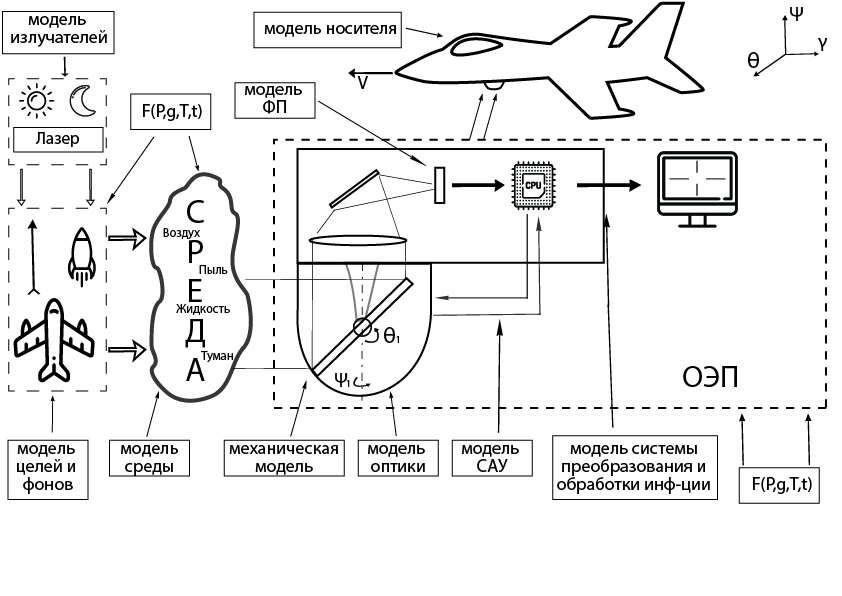
\includegraphics[width=0.8\linewidth]{oep_sch} 
	\caption{Функциональная схема обобщённой модели ОЭП}
	\label{fig:oep_sch}
\end{figure}


\section{Разработка математической модели} \label{sec:ch2/sec3}

\section{Верификация параметров} \label{sec:ch2/sec4}

\section{Оценки декомпозируемости каналов управления, основанные на анализе устойчивости и качества регулирования каналов управления с учетом перекрестных связей в частотной области} \label{sec:ch2/sec5}

\section{Синтез регуляторов частотным методом} \label{sec:ch2/sec6}

\section{Разработка КИМ и исследование динамики пространственной модели} \label{sec:ch2/sec7}

\section{Разработка алгоритмов управления БОЭП} \label{sec:ch2/sec8}

\section{Разработка компьютерной имитационной модели} \label{sec:ch2/sec9}

\section{Макетные испытания} \label{sec:ch2/sec10}

\section{Выводы по главе} \label{sec:ch2/sec11}



ll
